\documentclass[a4paper,11pt]{article}
\usepackage{graphicx}


\title{High Level Design Document \\ Bin-packing VM Consolidation Algorithm}
\author{Atchutuni Bhavana 13MCMT01  \\ Terli Venkatesh 13MCMT55 \\ Surineni Sampath Kumar 13MCMT49}


\date{}

\begin{document}
\maketitle
\pagebreak
\tableofcontents
\pagebreak

\section{Introduction}
The purpose of this document is to depict the high level
design and the data flow diagram of bin packing
vm consolidation algorithm project.
\section{Modules in the system}
Our system is divided into 3 modules. They are
\begin{enumerate}
\item \textbf{ User Interface }

This module is the main interface to the user and is responsible for building, editing and updating the GUI.
\item \textbf{ Parser }

This module reads the input from file, parses it and initializes PM’s and VM’s as specified in it.
\item \textbf{ PM modifier }

This module is responsible for adding virtual machines(VM) and doing modifications to Physical Machines(PM)s. This is also responsible for consolidation operation.

\end{enumerate}

\begin{figure}[h]
\centering
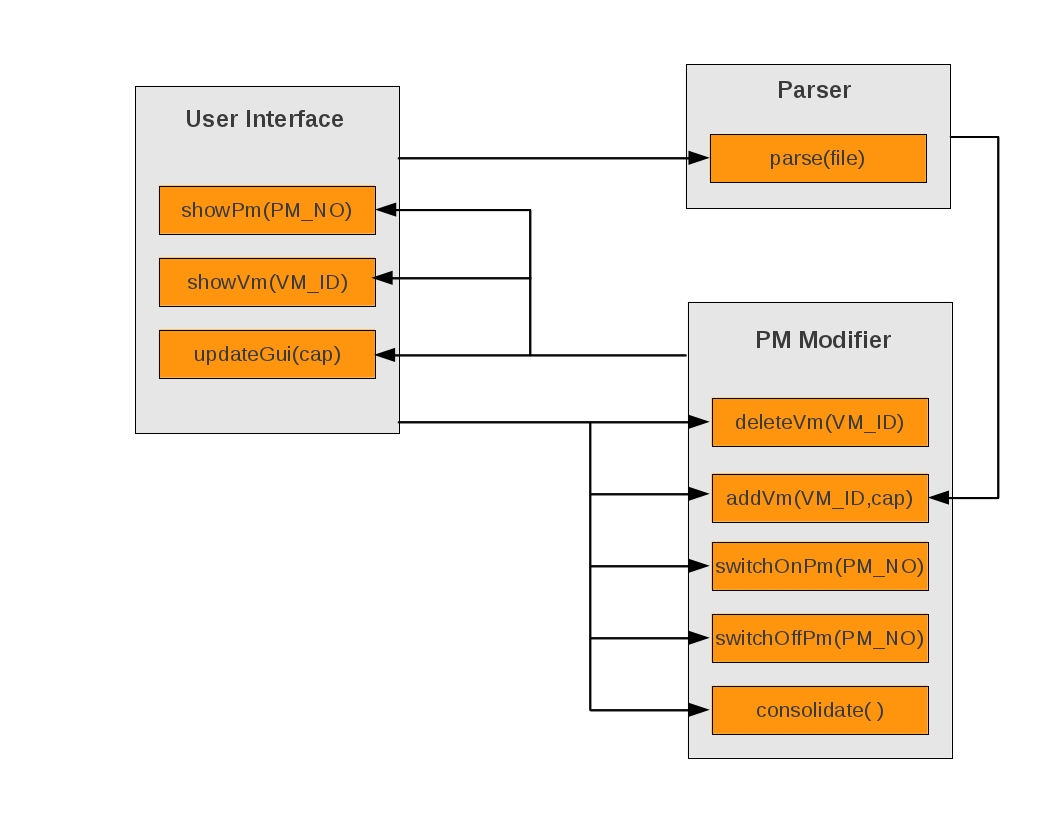
\includegraphics[height=9cm]{images/intrfc.jpg} 
\caption{Interfaces between modules}
\label{fig:interfaces}

\end{figure}

\pagebreak
\subsection{Data flow diagram}

\begin{figure}[h]
\centering
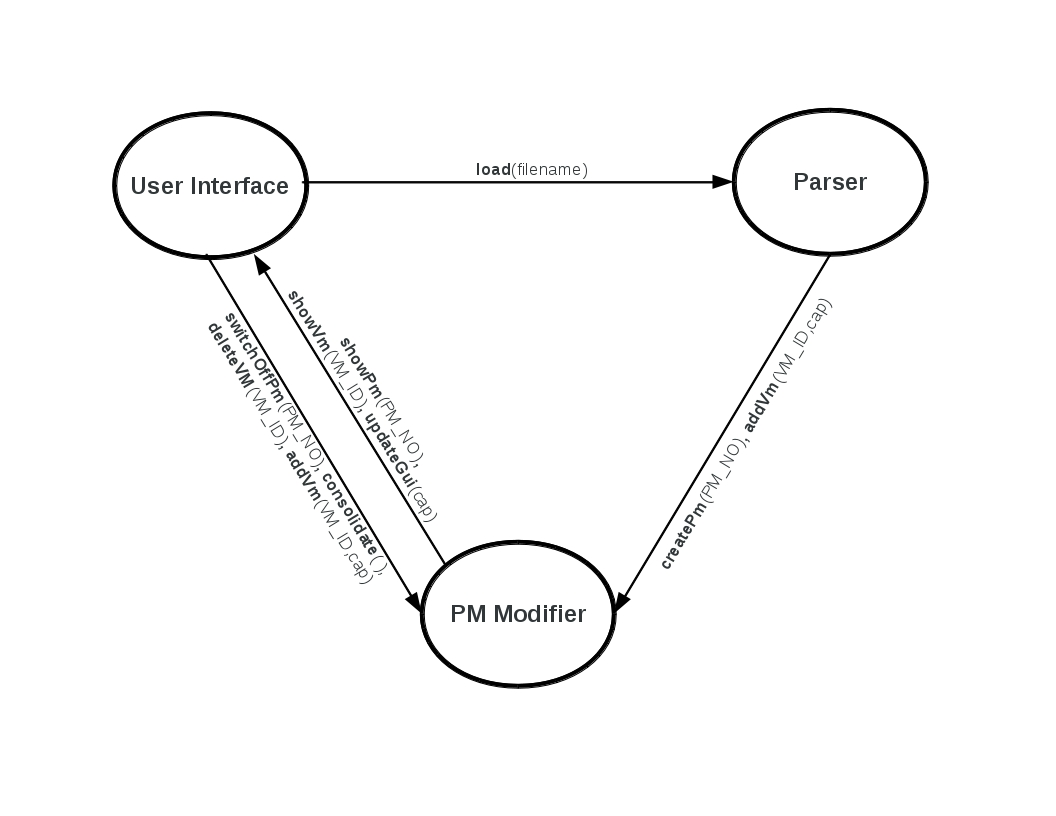
\includegraphics[height=11cm]{images/dfd.jpg}
\caption{Data flow diagram}
\label{fig:modules}

\end{figure}




\subsection{API Specification}
\subsubsection{Modules of the architecture }
\textbf{Main module}
\begin{itemize}
\item \textbf{Functionality}

This module is the central interface between all others modules. All the communications between the modules must pass through this module. This provides a 
standard interface for all modules to communicate with each other.

\item \textbf{Interface Description}

\textbf{callParser()}
  
\begin{tabbing}
\hspace*{4cm}\= \kill
 \textit{Purpose} \> : All the calls to Parser from other modules pass \\ \>through this function.\\
  \textit{Input Parameter} \> : fuction to be called in parser module and required parameters. \\
  \textit{Output Parameter} \> : none \\
  \textit{Called by} \> : User Interface module \\
  \textit{Calls} \> : all the fuctions in Parser module\\
\end{tabbing}
\textbf{callUI()}
  
\begin{tabbing}
\hspace*{4cm}\= \kill
 \textit{Purpose} \> : All the calls to User Interface module from other modules pass \\ \>through this function.\\
  \textit{Input Parameter} \> : Fuction to be called in User Interface module and \\ \>required parameters. \\
  \textit{Output Parameter} \> : none \\
  \textit{Called by} \> : PM modifier \\
  \textit{Calls} \> : All the fuctions in Parser module\\
\end{tabbing}
\textbf{callPmModifier()}
  
\begin{tabbing}
\hspace*{4cm}\= \kill
 \textit{Purpose} \> : All the calls to PM Modifier module from other modules pass \\ \>through this function.\\
  \textit{Input Parameter} \> : Fuction to be called in PM modifier module and \\ \>required parameters. \\
  \textit{Output Parameter} \> : none \\
  \textit{Called by} \> : Parser moduler and User Interface module \\
  \textit{Calls} \> : All the fuctions in PM Modifier module through Main module\\
\end{tabbing}
\end{itemize}
\textbf{User Interface Module}
\begin{itemize}
 \item \textbf{Functionality}
 
 The main purpose of this module is to take input from the user and reflect the system state to the user.
  \item \textbf{Interface Description}
  \end{itemize}
  \textbf{showPm(PM\textunderscore NO)} 
%\begin{tabbing}
%\hspace*{2cm}\=\hspace*{3cm}\= \kill
%column1a \> column2a \> column3a \\
%column1b \> column2b \> column3b
%\end{tabbing}
\begin{tabbing}
\hspace*{4cm}\= \kill
 \textit{Purpose} \> : This function takes the input from the parse file and \\ \>creates a UI element for PM and displays it.\\
  \textit{Input Parameter} \> : PM number \\
  \textit{Output Parameter} \> : none \\
  \textit{Called by} \> : PM modifier module through Main module
  
\end{tabbing}
%\begin{figure}[h]
%\centering
%\includegraphics[height=7cm]{images/init.png}
%\caption{Initial User Interface}
%\label{fig:GUIinit}
%\end{figure}
\begin{figure}[h]
\centering
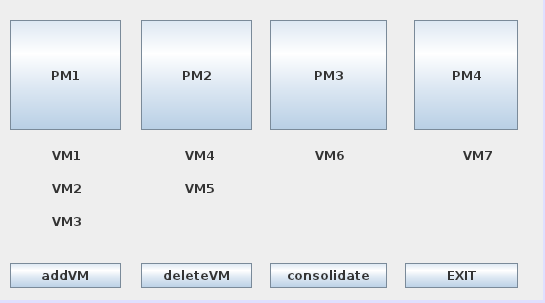
\includegraphics[height=7cm]{images/GUI.png}
\caption{Main user interface}
\label{fig:GUI}
\end{figure}
\textbf{showVm(VM\textunderscore ID)}  
\begin{tabbing}
\hspace*{4cm}\= \kill
 \textit{Purpose} \> :This function takes the input from the parse file and \\ \>creates a UI element for VM and displays it in corresponding PM.\\
  \textit{Input Parameter} \> : VM ID \\
  \textit{Output Parameter} \> : none \\
  \textit{Called by} \> : PM modifier module through Main module
  
\end{tabbing}
\textbf{updateGui()}  
\begin{tabbing}
\hspace*{4cm}\= \kill
 \textit{Purpose} \> :The purpose of this function is to update the GUI after\\ \> a modification has been done to a PM like adding a VM \\ \>or deleting a VM.\\
  \textit{Input Parameter} \> : none \\
  \textit{Output Parameter} \> : none \\
  \textit{Called by} \> : PM modifier module
  
\end{tabbing}
\textbf{Parser}
\begin{itemize}
\item \textbf{Functionality}

The aim of this module is to parse a text file specified by the user, extract the information about PM's and VM's in it.
It then initializes the PM's and adds VM's to them by the help of PM modifier module.

\item \textbf{Interface Description}

\textbf{parse(filename)}
  
\begin{tabbing}
\hspace*{4cm}\= \kill
 \textit{Purpose} \> :The purpose of this function is to parse the file specified by the \\ \>user and extract information about PM's and VM's.\\
  \textit{Input Parameter} \> : file path specified by the user \\
  \textit{Output Parameter} \> : none \\
  \textit{Return Value} \> : If the file is not in the specified format it would display \\ \>\textbf{wrong file format} message \\
  \textit{Called by} \> : User Interface module through Main module \\
  \textit{Calls} \> : createPM and addVM functions of PM modifier\\
\end{tabbing}
\end{itemize}
\textbf{PM modifier}
\begin{itemize}
\item \textbf{Functionality}

The operations of this module includes adding VM's to PM, calculating the residual capacity and consolidation.

\item \textbf{Interface Description}


\textbf{addVm(VM\textunderscore ID, cap)}
  
\begin{tabbing}
\hspace*{4cm}\= \kill
 \textit{Purpose} \> : The purpose of this function is to add VM's to the PM as specified\\ \> by the parser.\\
  \textit{Input Parameters} \> : VM ID and VM capacity. \\
  \textit{Output Parameter} \> : none \\
  \textit{Return Value} \> : If there is no enough space to add VM to a PM it outputs \\ \>\textbf{No enough space} message\\
  \textit{Called by} \> : Parser module through Main module \\
  \textit{Calls} \> : showVm of User Interface Module through Main module.\\
\end{tabbing}

\textbf{deleteVm(VM\textunderscore ID)}
  
\begin{tabbing}
\hspace*{4cm}\= \kill
 \textit{Purpose} \> : The purpose of this function is to delete a VM specified by the user.\\
  \textit{Input Parameters} \> : PM number in which VM resides and VM ID. \\
  \textit{Output Parameter} \> : none \\
 \textit{Called by} \> : User Interface module \\
  \textit{Calls} \> : none.\\
\end{tabbing}
\pagebreak
\textbf{switchOffPm(PM \textunderscore NO)}
  
\begin{tabbing}
\hspace*{4cm}\= \kill
 \textit{Purpose} \> : The purpose of this function is to switch off a PM specified by user.\\
  \textit{Input Parameters} \> : PM number. \\
  \textit{Output Parameter} \> : none \\
  \textit{Return Value} \> : Displays \textbf{It is not possible to switch off this PM at this time} if \\ \>switching off was not successful. \\
  \textit{Called by} \> : User Interface module through Main module \\
  \textit{Calls} \> : updateGui() through Main module.\\
\end{tabbing}
\textbf{switchOnPm(PM\textunderscore NO)}
\begin{tabbing}
\hspace*{4cm}\=\kill
\textit{Purpose}\>: The purpose of this function is to switch on a PM specified by user. \\
\textit{Input Parameters}\>: PM number.\\
\textit{Output Parameters}\>: none\\
\textit{Return Value}\>:\\
\textit{Called by}\>: User Interface module through Main module\\
\textit{Calls}\>: updateGui() through Main module.\\
\end{tabbing}

\textbf{consolidate( )}
  
\begin{tabbing}
\hspace*{4cm}\= \kill
 \textit{Purpose} \> : The purpose of this function is to run Bin packing algorithm and \\ \> consolidate all the VM's into minimum number of PM's.\\
  \textit{Input Parameters} \> : none \\
  \textit{Output Parameter} \> : none \\
    \textit{Called by} \> : User Interface module through Main module \\
  \textit{Calls} \> : none.\\
\end{tabbing}
\end{itemize}

\end{document}